\documentclass{article}
\usepackage{fancyhdr,booktabs}
\usepackage{amsmath}
\usepackage{float}
\usepackage{graphicx}
\usepackage{indentfirst}
\usepackage{geometry}

\begin{document}

\section{Numerical Methods}
\section{Confusion problem}

Given a waveform under specetiem with non-zero deformation parameter, we need to decide which waveform under Kerr specetime is most similar to it.

If we restrict ourselves to equatorial motion, set the initial $t$ and $\phi$ to 0 taking advantage of symmetry and set initial $r=r_{max}$ imposing the phase to match, orbital eccentricity $e$, semilatus rectum $p$, BH mass $M$ and BH spin $a$ are the parameters that determine the motion.

According to , orbits with same orbital frequency $\omega_r$ and $\omega_\phi$ can generate most similar gravitational waveforms. Here we check this result by lookinf at overlaps between waveforms with ($\delta_1,\, a,\, M,\, e,\, p$) = (0.2, 0.5, , 0.5, 6).

First we look at overlap distribution on a relatively large range of (e, p).

Then take a closer look at the distribution near (e,p) with same orbital frequency. Note that the same orbital frequency with respect to t can result in largest overlap while the same orbital frequency with respect to $\tau$ cannot.

\begin{figure}[!htb]
	\centering
	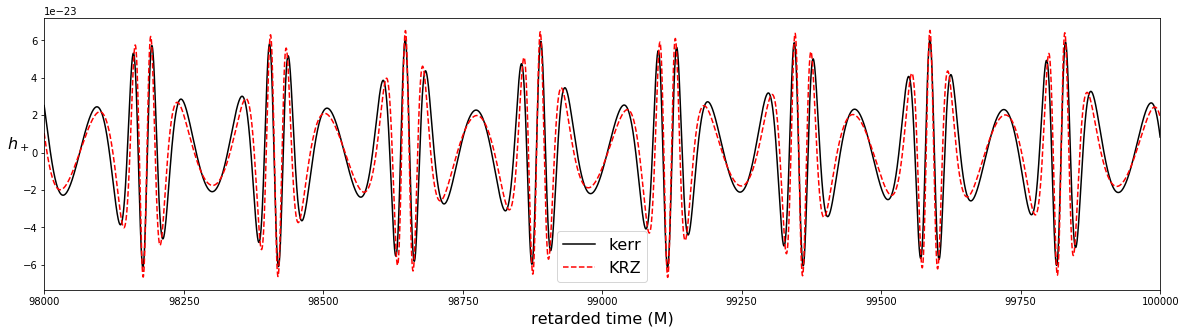
\includegraphics[width=16cm]{krz_kerr_wave.png}
	
	\caption{Comparison between waveforms of $h_+$ with respect to retarded time in units of central black hole mass $M$. The black solid line is the waveform under $\delta_1=0.2$, e=0.5,p=6. The red dashed line is the waveform under $\delta_1=0$ and e, p adapted so that the orbital frequencies with respect to t $\omega^{(t)}_r$ and $\omega^{(t)}_\phi$ are the same as that of the orbit under d1=0.2, e=0.5, p=6. The green dotted line is the waveform under $\delta_1 =0$ and e, p adopted so that $\omega^{(\tau)}$s are the same . The spin of the central black hole is 0.5M.}
	\label{range}
\end{figure}	
	
Therefore we regard waveforms in Kerr spacetime with same orbital frequencies as best matches to waveforms in non-Kerr space time under KRZ parametrization.

Fig. shows the overlap distrobution...

As Fig. suggest, the confusion problem still exists in KRZ parametrization. The deformation parameter $\delta_1$ is kind of degenerated with   in Kerr spacetime. This resulted can also be found by looking at covariance matrix as discussed in next section
\section{Restriction on deformation parameter by future LISA task}
\end{document}